\documentclass[sigplan,anonymous,review]{acmart}
\usepackage{booktabs}
\usepackage{tabularx}
\usepackage{microtype}
\usepackage{tikz}
\usepackage{balance}
\usetikzlibrary{arrows.meta,positioning}
\settopmatter{printfolios=true,printacmref=false}
\setcopyright{none}
\renewcommand\footnotetextcopyrightpermission[1]{}
\acmConference[EuroSys '27]{Twenty-Second European Conference on Computer Systems}{April 19--23, 2027}{Rabat, Morocco}
\acmYear{2027}
\title[Joggle]{Joggle: Malleable Compilation with a Progressive Intermediate Representation}
\author{Anonymous Author(s)}
\affiliation{\institution{Anonymous}}
\ccsdesc[500]{Software and its engineering~Compilers}
\ccsdesc[300]{Computer systems organization~Embedded systems}
\begin{document}
\begin{abstract}
Research experiments increasingly change model semantics, representations,
optimization procedures, and artifact interfaces together. Modern compilers
provide strong extension points for each concern, but a changing experiment
still has to coordinate their distinct executable contracts. We present
Joggle, a compiler substrate with a progressive intermediate representation:
individual function bodies expose implementation detail while the surrounding
program retains one typed editing model. Compiler procedures are also ordinary
inspectable functions. A researcher can derive a definition and its private
call closure in a separate module, edit the copied algorithm, and run it over
a model through the same checked
execution boundary. We test these mechanisms on neural inference, where
Joggle completely relates 13 of 14 pinned ONNX models and produces ten
numerically checked C artifacts. A general loop policy improves a
MobileNetV2 generated-C pilot by 26.5\%, while the resulting artifact remains
12.24$\times$ slower than adjacent one-thread ONNX Runtime. The matched
cross-system revision experiment needed to establish lower coordination cost
remains open.
\end{abstract}
\keywords{malleable compilation, progressive intermediate representation, compiler infrastructure, hardware-software co-design, program optimization}
\maketitle
\section{Introduction}
A hardware specialization rarely ends at a kernel. Consider adding a packed
low-precision projection to an inference processor. A complete experiment needs
to recognize the source computation, preserve a portable meaning, represent
packed constants, expose the loops that a structural policy must change, decide
when the target implementation applies, and construct a callable artifact. A
revision to the group size or packing contract changes several of these
decisions together. Although the proposed primitive is local, the research
object is a vertical slice of the compiler.

Modern compiler stacks make every part of this slice programmable. MLIR exposes
extensible operations, types, interfaces, conversions, and transformations
\cite{lattner2021mlir,lucke2025transform}. TVM composes Relax functions,
TensorIR functions, schedules, external calls, and runtime modules
\cite{chen2018tvm,lai2025relax}. Exo externalizes accelerator instructions,
special memories, and trusted schedule rewrites \cite{ikarashi2022exo}, while
TileLang provides a concise tiled-program boundary \cite{wang2025tilelang}.
These divisions are valuable: each representation and interface carries
invariants needed for mature optimization.

MLIR even supports runtime-defined dialects and IRDL descriptions; partial
conversion retains mixed operations in one generic IR
\cite{mlirDynamicDialectDocs,mlirIrdlDocs,mlirConversionDocs}. The missing
property is therefore neither extensibility nor mixed-level representation.
Rather, the projection above may be implemented across a frontend relation,
graph legalization, tensor function, schedule, target hook, runtime
registration, and build rule, each with its own checking or deployment event.
We call this potential mismatch between a vertical research concept and its
independently governed extension contracts \emph{extension fragmentation}.
It is a hypothesis about revisions, not a claim that multiple IRs are
intrinsically costly. Figure~\ref{fig:mismatch} depicts the contracts that the
matched evolution study must audit.

This mismatch is becoming more common. Model families continue to introduce
local fusions and structures faster than fixed rule sets absorb them
\cite{wu2025plus}. Emerging formats couple storage, access, conversion, and
scheduling \cite{wang2024ladder}; tensor-ISA descriptions increasingly generate
backend components \cite{jain2026act}. Handwritten policies now coexist with
search, synthesis, and generated compiler changes. These trends do not make
existing stacks obsolete. They make the compiler itself a moving research
object and broaden the set of producers that need an inspectable, bounded, and
recoverable way to change it.

We call that systems property \emph{malleability}: the ability to change where
and how implementation detail enters a program without reconstructing the
surrounding compilation path. Malleability is neither generality nor performance
portability. It requires continuity of program identity, portable fallback,
dependency lifecycle, failure containment, and artifact construction while a
vertical extension evolves.

Joggle treats the compiler as a research instrument, not a fixed sequence of
optimizers. Its stable host owns structural validity, edit authority, and
publication; installed modules own the experimental meaning, applicability,
implementation, and artifact policy. A consumer requests only the detail it
can accept, so committing to a new format or target does not force every
function through the same representation change. The program remains the
inspectable object of the experiment while those decisions evolve.

Joggle realizes this property with two coupled mechanisms. First, a
\emph{progressive intermediate representation} exposes implementation detail
locally. An abstract relation may acquire a reusable tensor body, become
explicit loops, or bind an external implementation while other functions remain
abstract. Every state retains the surrounding function identity and the same
typed \texttt{Fn/Blk/Op/Val} object model, verifier, printer, and editing
interface. Replaced operations and values receive new generations, making
stale handles invalid. Second, compiler procedures themselves use this
inspectable function representation. Analysis, selection, structural edits,
representation policy, and generation can be composed as typed functions.
Deriving an inactive copy permits a local edit to the procedure while its
original remains callable. The compiler definition and the target model are
separate \texttt{Mod} values of the same IR type; a checked function call connects
them without inserting compiler code into the emitted model. Module
installation and verified transactions govern dependencies and mutation.

Joggle deliberately does not replace specialized IRs or claim the optimization
maturity of production compilers. The current evaluation tests the prerequisites
for a malleable path: mixed representation reach, cross-role extension breadth,
checked artifact closure, and bounded failure. Revision coordination and
generated-code quality are reported as separate outcomes. This separation
prevents short source paths from being misreported as usability and prevents
fast kernels from being misreported as a complete research workflow.

This paper makes three contributions:

\begin{enumerate}
\item
\textbf{Progressive IR}, in which abstract relations, reusable
tensor bodies, explicit loops, storage decisions, and external calls remain
locally exposable states of one typed program rather than mandatory
whole-program stages.

\item
\textbf{Derivable compiler functions} that expose analysis, policy,
transformation, and generation bodies to the existing clone/edit/invoke
facilities, with typed execution over a separate target program.

\item
\textbf{An implemented substrate and evidence boundaries} covering real-model
reach, cross-role extension breadth, checked artifacts, and generated-code
quality. A cross-system revision and a useful optimized compiler procedure
remain necessary tests of malleability.

\end{enumerate}

\begin{figure*}[t]
\centering
\resizebox{\textwidth}{!}{%
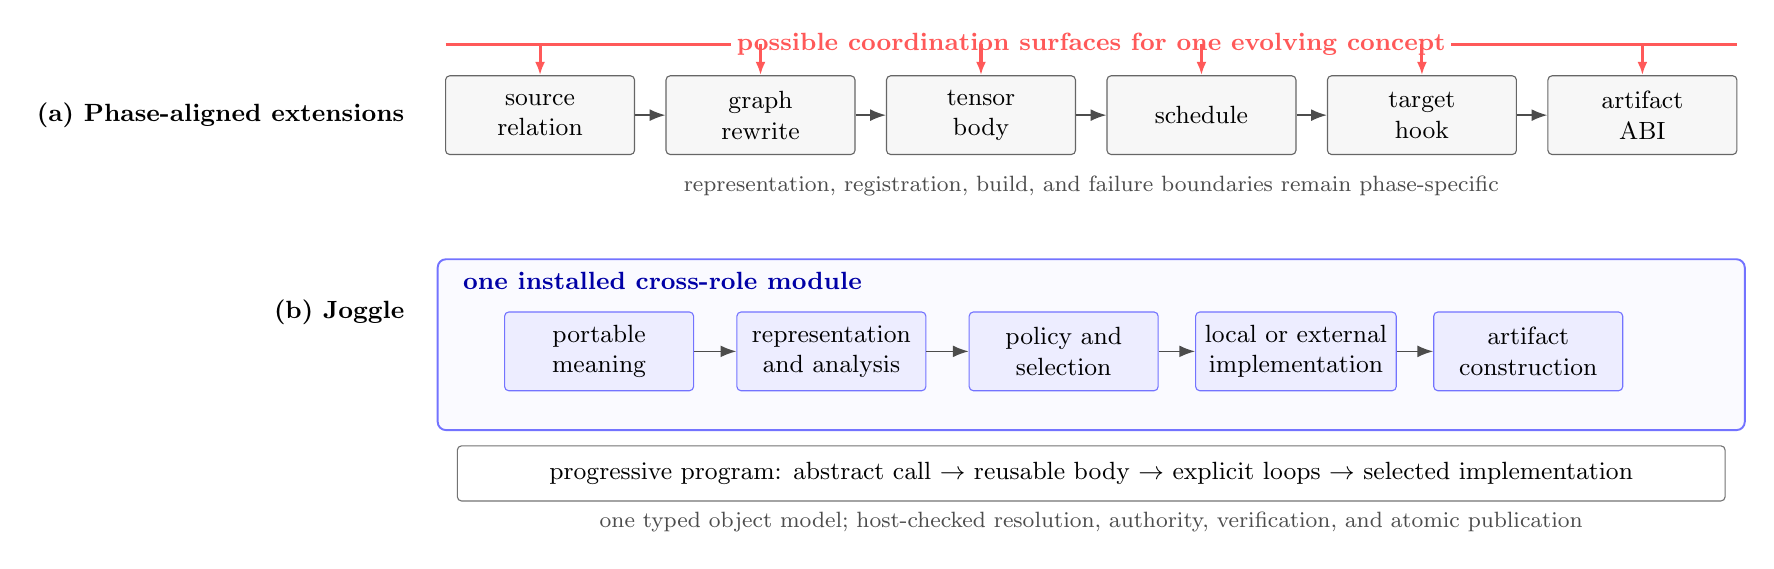
\begin{tikzpicture}[
  role/.style={draw=black!60, rounded corners=1.5pt, fill=black!3,
               minimum width=24mm, minimum height=10mm, align=center,
               font=\small},
  jrole/.style={role, fill=blue!7, draw=blue!55},
  link/.style={-{Latex[length=2mm]}, line width=.55pt, black!70},
  touch/.style={line width=1.1pt, red!65},
  lab/.style={font=\small\bfseries, anchor=east}
]
\node[lab] at (-.25,1.45) {(a) Phase-aligned extensions};
\node[role] (src) at (1.35,1.45) {source\\relation};
\node[role] (graph) at (4.15,1.45) {graph\\rewrite};
\node[role] (tensor) at (6.95,1.45) {tensor\\body};
\node[role] (sched) at (9.75,1.45) {schedule};
\node[role] (target) at (12.55,1.45) {target\\hook};
\node[role] (abi) at (15.35,1.45) {artifact\\ABI};
\draw[link] (src) -- (graph);
\draw[link] (graph) -- (tensor);
\draw[link] (tensor) -- (sched);
\draw[link] (sched) -- (target);
\draw[link] (target) -- (abi);
\draw[touch] (0.15,2.35) -- (16.55,2.35);
\node[fill=white, inner sep=2pt, font=\small\bfseries, text=red!65]
  at (8.35,2.35) {possible coordination surfaces for one evolving concept};
\foreach \n in {src,graph,tensor,sched,target,abi}
  \draw[touch,-{Latex[length=1.7mm]}] (\n.north |- 0,2.35) -- (\n.north);
\node[font=\footnotesize, text=black!70] at (8.35,.55)
  {representation, registration, build, and failure boundaries remain phase-specific};

\node[lab] at (-.25,-1.05) {(b) Joggle};
\draw[rounded corners=3pt, fill=blue!2, draw=blue!55, line width=.7pt]
  (0.05,-2.55) rectangle (16.65,-.38);
\node[anchor=west, font=\small\bfseries, text=blue!65!black]
  at (.25,-.65) {one installed cross-role module};
\node[jrole] (meaning) at (2.10,-1.55) {portable\\meaning};
\node[jrole] (repr) at (5.05,-1.55) {representation\\and analysis};
\node[jrole] (policy) at (8.00,-1.55) {policy and\\selection};
\node[jrole] (impl) at (10.95,-1.55) {local or external\\implementation};
\node[jrole] (artifact) at (13.90,-1.55) {artifact\\construction};
\draw[link] (meaning) -- (repr);
\draw[link] (repr) -- (policy);
\draw[link] (policy) -- (impl);
\draw[link] (impl) -- (artifact);
\node[draw=black!55, rounded corners=1.5pt, fill=white, minimum width=16.1cm,
      minimum height=7mm, font=\small, align=center] at (8.35,-3.10)
  {progressive program: abstract call $\rightarrow$ reusable body $\rightarrow$
   explicit loops $\rightarrow$ selected implementation};
\node[font=\footnotesize, text=black!70] at (8.35,-3.72)
  {one typed object model; host-checked resolution, authority, verification, and atomic publication};
\end{tikzpicture}
}%
\caption{The unit-of-change hypothesis. Phase-aligned interfaces offer
specialized invariants but may split one evolving concept across separately
governed objects (a). The arrows mark possible interfaces, not six mandatory
edits in every system or revision. Joggle keeps the roles distinct as
typed functions while placing their lifecycle in one module and exposing
implementation detail locally in one program (b). This is the paper's
architectural claim; Section~5 tests its implemented prerequisites and keeps the
still-missing revision-coordination result separate from artifact and
performance evidence.}
\Description{Two compiler organization diagrams. The first shows one co-design
change touching source relation, graph rewrite, tensor body, schedule, target
hook, and artifact ABI boxes. The second places corresponding roles inside one
installed Joggle module above a progressive-program rail, with host checks
underneath.}
\label{fig:mismatch}
\end{figure*}

\section{Motivation and hypothesis}
\subsection{Vertical innovation does not follow compiler phases}
Our frozen example begins with an ordinary \texttt{Conv--Add--Relu} model. At
S0, an external NCHW/OIHW convolution replaces only \texttt{Conv}; broadcast
bias addition and ReLU remain portable. At S1, the target consumes OIHW2-packed
weights and accepts only even input-channel counts. The
source model and result type must stay fixed, while payload materialization,
applicability, and the odd-channel fallback change. At S2, the target ABI adds a
bias pointer and an activation selector. The eligible \texttt{Conv--Add--Relu}
chain can now use one target call, but the fallback must still compute the same
result through portable bodies. These are successive revisions to one
specialization, not three independent operator implementations.

The difficulty is visible before performance tuning. A source relation alone
cannot construct the packed constant or native entry ABI; a kernel alone cannot
decide whether a model occurrence is eligible or preserve its portable
fallback. An optimizer must inspect the represented producer--consumer chain,
and an artifact builder must agree with its selected call and payload layout.
Changing the packing factor or epilogue contract therefore revisits several
compiler roles while leaving the application program unchanged. The relevant
cost is how many independently validated extension contracts must be
coordinated across that revision, not the number of source files or IR levels.

The compiler procedure can itself become the research object. For instance,
the same model may need a changed applicability test, a modified access
analysis, and a different C emitter. A selector script can call these
procedures, but calling a procedure to edit a model does not edit the
procedure's own algorithm. If a researcher wishes to specialize the analysis
or generation function, its definition must remain inspectable and executable
after the edit. It must also stay outside the model's artifact: in a regression
using a typed model, copying compiler code into the
target program makes C preparation try to compile that code as model
computation. The working route holds compiler definitions and model
computation in distinct \texttt{Mod} values with one function representation
and a checked invocation between them.

Recent work exposes the same coupling in different domains. Ladder links
low-precision storage to access, conversion, and scheduling
\cite{wang2024ladder}; ACT derives backend components from a tensor-ISA
description \cite{jain2026act}. PluS and Axon enlarge graph or multi-level
optimization spaces \cite{wu2025plus,kothari2026axon}, while Autocomp and Argus
make generated candidates depend on executable feedback
\cite{hong2025autocomp,mai2026argus}. None is a Joggle baseline for this task.
They motivate a compiler substrate in which a changing concept can be checked
from source recognition through artifact closure.

\subsection{What existing boundaries buy---and what they separate}
The closest alternatives already solve much of this problem. MLIR dialects and
interfaces state invariants explicitly; dynamic dialects and IRDL permit
runtime vocabulary definitions, while partial conversion permits mixed legal
and unconverted operations
\cite{lattner2021mlir,mlirDynamicDialectDocs,mlirIrdlDocs,mlirConversionDocs}.
Its Transform dialect represents rewrite intent as a composable program over
mutable payload IR, with handle invalidation and pre/postconditions
\cite{lucke2025transform,mlirTransformDocs}.
Exo 2 constructs new scheduling operations from trusted primitives
\cite{ikarashi2024exo2}; AnyDSL partially evaluates reusable higher-order
programs, and weval derives compiled execution from an interpreter body
\cite{leissa2018anydsl,fallin2025weval}. Transforming a transformation,
staging a procedure, and reusing its implementation are therefore established
ideas. Joggle must demonstrate a useful consequence of applying its ordinary
function representation across compiler roles, rather than claim those ideas
from function syntax alone.
TVM is a stronger counterexample to a claim about ``too many IRs'': one
\texttt{IRModule} contains Relax and TensorIR functions. Cross-level calls,
runtime modules, and \texttt{PackedFunc}s connect compilation to deployment
\cite{lai2025relax,tvmArchitectureDocs,tvmRuntimeDocs}. Spoofax also packages
syntax, analysis, transformation, generation, and editor services as a language
project \cite{kats2010spoofax}. These boundaries provide reusable invariants,
partial lowering, and mature ecosystems; their existence is not itself the
problem.

The open question is what happens when the S0 specialization changes twice.
In MLIR, a transform program and dialect-defined payload can share the same
generic operation storage but retain distinct executable contracts. In TVM,
a Relax relation, a TensorIR body or
external call, and a runtime module can share a container and call interface
without sharing one editable body representation or one extension upgrade
event. Spoofax packages cross-role language definitions, but its project unit
does not by itself provide transactional edits over a live native-artifact
compiler program. ONNX-MLIR and IREE offer staged native deployment
\cite{jin2020onnxmlir,ireeDocs}; Exo and TileLang provide richer, more
controllable kernel construction \cite{ikarashi2022exo,wang2025tilelang}.
None of these observations proves that Joggle requires less engineering effort.
They identify a testable difference: whether a representation-and-ABI revision
can be validated and published through fewer independently coordinated
framework boundaries while retaining the same source and fallback.

Joggle explores whether the unit of change can instead match the concept being
changed. The structural program and its safety rules remain stable; a module
generation carries the concept's semantics, selection, structural policy, and
artifact actions. Each consumer determines how much of that program to expose.
This design does not collapse every invariant into a universal tensor IR:
modules may impose stronger local meaning and checks where a target or
optimization requires them.

\subsection{Requirements for malleable compilation}
The proposed change unit must satisfy five requirements.

\paragraph{Local exposure.}
Implementation detail must be introduced per function rather than through a
mandatory whole-program transition. Abstract and explicit regions must coexist
and remain inspectable through one public identity.

\paragraph{Cross-role lifecycle.}
The vocabulary, meaning, analyses, transformations, target decisions, and
artifact actions of one research concept must be installable, versioned, and
replaceable as one dependency unit. Source-only and native components may have
different build costs, but they must not acquire unrelated lifecycle models.

\paragraph{Editable compiler behavior.}
The analysis, selector, representation procedure, transform, and generator
must be inspectable at the function-body level. A derived procedure must
execute against a target program without becoming part of that program's
artifact. This requires an explicit boundary between two values of the same
\texttt{Mod} type, not a new category of pass or a second IR.

\paragraph{Bounded change.}
Modules inspect and transform live program structure under bounded access. The
host must enforce type compatibility, mutation
authority, verification, rollback, and dependent-module validation for
handwritten, searched, synthesized, and generated changes alike.

\paragraph{Artifact closure.}
The final source, payloads, declarations, symbols, and entry ABI must derive
from the represented program. An out-of-band harness that silently reconstructs
these decisions would merely move extension fragmentation past the compiler.

\subsection{Hypothesis and scope}
Our hypothesis is that locally exposed function bodies and derivable compiler
functions reduce the coordination required to change a compiler experiment.
The first prediction is a verified model containing abstract relations,
portable bodies, and selected implementations without a whole-program
representation migration. The second is a derived compiler procedure that can
reuse analysis, change its own algorithm, and act on a separate model while
the source procedure remains executable. The third is a matched revision path
with fewer independently governed contracts or a useful optimized procedure
at acceptable execution cost. The current evidence establishes representation,
typed invocation, extension breadth, artifacts, and failure containment.
It does not yet establish the third prediction.

The hypothesis fails if progressive states are separate editing models hidden
behind attributes, if each new optimization requires a host primitive, if
errors are deferred beyond comparable specialized IR checks, or if artifact
construction relies on an undocumented ABI. It also has a practical boundary:
a malleable compiler that cannot transform representative programs is not a
useful substrate. Generated-code quality remains an independent result---a
shorter change path does not excuse slow output, and a fast kernel does not
establish a complete research workflow.

\section{Progressive intermediate representation and compiler functions}
\subsection{One program, increasing implementation detail}
Joggle programs contain seven public concepts: modules, functions, blocks,
operations, values, structural types, and open attributes. There is no separate
graph object, schedule tree, pass class, or target node in the host. Calls and
structured control flow are operations. Tensor shape and numeric format are
types. Source schema fields, target facts, and analysis results are attributes
only when they are properties of represented objects rather than hidden global
state.

Progressive IR changes function bodies, not the identity of the program. A
source call may remain abstract while graph-scale transformations operate on
calls. A consumer that rejects it requests more detail, causing a portable body
to be instantiated as explicit loops and scalar operations. Alternatively, a
selection policy may bind a type-compatible external implementation without
first exposing that body. These choices are per call, so one program may contain
both states. Figure~\ref{fig:progressive} traces this behavior through Joggle's
checked \texttt{edge} example rather than presenting three disconnected toy
IRs.

The invariant is not that all abstraction levels are equally convenient.
Rather, every exposed state remains a typed function program accepted by the
same verifier and edit API. Specialized modules may establish stronger local
contracts, but crossing that contract does not require moving the whole model
into another host representation.

\begin{figure*}[t]
\centering
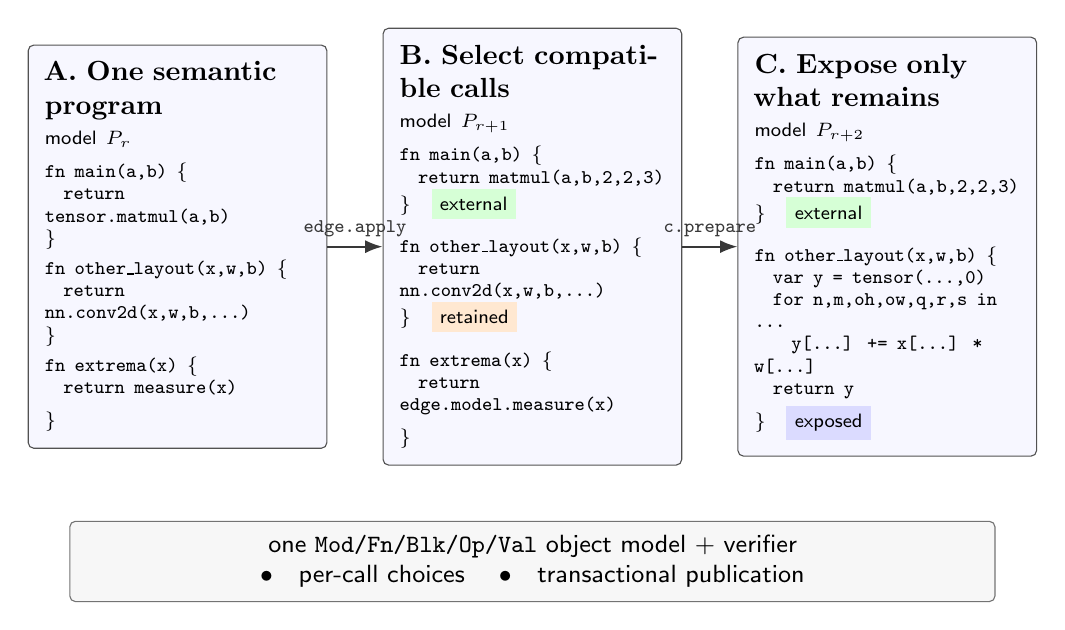
\begin{tikzpicture}[
  state/.style={draw=black!68, rounded corners=2pt, fill=blue!3,
                text width=.278\textwidth, minimum height=48mm,
                align=left, inner sep=6pt},
  flow/.style={-{Latex[length=2.2mm]}, line width=.7pt, black!78},
  invariant/.style={draw=black!55, rounded corners=2pt, fill=black!3,
                    align=center, inner sep=5pt, text width=.94\textwidth,
                    font=\sffamily\small}
]
\node[state] (source) {
  \textbf{A. One semantic program}\\[-1pt]
  {\scriptsize \textsf{model} $P_r$}\\[4pt]
  {\ttfamily\scriptsize
  fn main(a,b) \{\\
  \ \ return tensor.matmul(a,b)\\
  \}\\[3pt]
  fn other\_layout(x,w,b) \{\\
  \ \ return nn.conv2d(x,w,b,...)\\
  \}\\[3pt]
  fn extrema(x) \{\\
  \ \ return measure(x)\\
  \}}
};
\node[state, right=7mm of source] (selected) {
  \textbf{B. Select compatible calls}\\[-1pt]
  {\scriptsize \textsf{model} $P_{r+1}$}\\[4pt]
  {\ttfamily\scriptsize
  fn main(a,b) \{\\
  \ \ return matmul(a,b,2,2,3)\\
  \}\quad{\sffamily\scriptsize\colorbox{green!16}{external}}\\[6pt]
  fn other\_layout(x,w,b) \{\\
  \ \ return nn.conv2d(x,w,b,...)\\
  \}\quad{\sffamily\scriptsize\colorbox{orange!18}{retained}}\\[6pt]
  fn extrema(x) \{\\
  \ \ return edge.model.measure(x)\\
  \}}
};
\node[state, right=7mm of selected] (prepared) {
  \textbf{C. Expose only what remains}\\[-1pt]
  {\scriptsize \textsf{model} $P_{r+2}$}\\[4pt]
  {\ttfamily\scriptsize
  fn main(a,b) \{\\
  \ \ return matmul(a,b,2,2,3)\\
  \}\quad{\sffamily\scriptsize\colorbox{green!16}{external}}\\[6pt]
  fn other\_layout(x,w,b) \{\\
  \ \ var y = tensor(...,0)\\
  \ \ for n,m,oh,ow,q,r,s in ...\\
  \ \ \ \ y[...] += x[...] * w[...]\\
  \ \ return y\\
  \}\quad{\sffamily\scriptsize\colorbox{blue!14}{exposed}}
  }
};
\draw[flow] (source) -- node[above, font=\ttfamily\scriptsize]
  {edge.apply} (selected);
\draw[flow] (selected) -- node[above, font=\ttfamily\scriptsize]
  {c.prepare} (prepared);
\node[invariant, below=7mm of selected] (inv) {
  one \texttt{Mod/Fn/Blk/Op/Val} object model + verifier
  \quad$\bullet$\quad per-call choices
  \quad$\bullet$\quad transactional publication};
\end{tikzpicture}
\caption{A checked mixed-state trace from \texttt{examples/edge}. The input
program contains only semantic calls (A). \texttt{edge.apply} selects external
matrix and multi-result implementations but rejects a convolution whose layout
predicate is incompatible, leaving that call semantic (B). \texttt{c.prepare}
then exposes the portable bodies that remain, shown here by the rejected
convolution's loops, while selected calls stay external (C). The excerpts omit
types and operands for space, but preserve the functions and decisions printed
by the implementation. This is a legal trace, not a mandatory whole-program
lowering pipeline.}
\Description{Three excerpts of one checked Joggle program. Initially all three
functions use semantic calls. Selection binds compatible matrix and multi-result
calls to external implementations while retaining an incompatible-layout
convolution. Preparation then expands the depicted convolution into loops. A
band below states that all revisions use the same object model and verifier.}
\label{fig:progressive}
\end{figure*}

\subsection{Capability-directed exposure}
Let $P_r$ be a verified program at revision $r$, $A(o)$ a consumer-supplied
capability predicate, and $I(o)$ the structurally type-compatible
implementations of call $o$. Preparation walks calls reachable from exported
functions and applies one of four actions:
\[
T(o)=
\begin{cases}
\mathit{retain}(o), & A(o);\\
\mathit{retarget}(o,i), & i\in I(o)\text{ is external};\\
\mathit{expand}(o,i), & i\in I(o)\text{ has a body};\\
\mathit{frontier}(o), & \text{otherwise}.
\end{cases}
\]
Selection among multiple members of $I(o)$ is a separate read-only typed
function. It may encode a rule, cost model, search result, or generated policy,
but may return at most one compatible member. Thus capability states what a
consumer can accept, while selection states which legal implementation it
prefers.

The transform collects a round's decisions before editing. An external
declaration retargets a call; a definition is cloned into the caller and its
arguments and results are rewired. New calls exposed by that body are considered
in the next round. Preparation returns a capability-closed program when no
reachable call remains outside $A$, or a typed frontier when no implementation
can make progress. Because arbitrary module bodies need not decrease a static
measure, Joggle does not claim unconditional termination: the caller supplies a
round bound, and exceeding it aborts the invocation.

For a successful transition $P_r\rightarrow P_{r'}$, the host establishes
three properties: $P_{r'}$ passes whole-program verification, every edit lies
within the invocation's authority, and the enclosing function remains in the
same program and object model. Replaced operations and values deliberately do
not retain handle identity. On ambiguity, an invalid expansion, nonconvergence,
or verification failure, the observable result is $P_r$. This transactional
boundary makes local exposure composable without pretending that arbitrary
rewrites are monotone.

The four actions may coexist in one artifact. A mature matrix operation can
remain a library call, a custom packed projection can select a device module,
and an uncommon elementwise call can expose into portable loops. No global
lowering event forces these choices to occur at the same abstraction level.

\subsection{Deriving and running compiler functions}
Compiler behavior uses ordinary typed \texttt{Fn} definitions. A policy may
inspect an existing analysis as a function, invoke it with a live \texttt{Mod},
clone its definition, and edit the copy's \texttt{Blk/Op/Val} body with the
same structural primitives used on model computation. The procedure's role
comes from its signature and callers: \texttt{fn(Mod)->dict} can be an
analysis, \texttt{fn(Mod,Op)->bool} a structural edit, and
\texttt{fn(Mod)->str} a generator. No host-side pass subclass identifies
these roles.

The distinction between a procedure and its subject is concrete. Let $S$
contain an installed source definition $f$, $K$ hold derived compiler
definitions, and $P$ hold model computation; each is a value of the public
\texttt{Mod} type. A derivation $D(S,f,e;K)$ creates a fresh definition $f_e$
in $K$ by cloning $f$ and applying an edit $e$ to the inactive copy. The
source $f$ in $S$ remains callable. An execution
$\mathit{invoke}(f_e,P)$ reads or edits $P$; $f_e$ is not appended to $P$.
With a read-only query, Joggle checks that the target snapshot is unchanged.
With a mutating call, the target is verified and either the new revision is
published or the original revision is restored. Code edits to $K$ and
program edits to $P$ are distinct transactions, not one implicit atomic
exchange. The caller must validate an independently edited $K$ before use.

The C++ embedding API accepts a live \texttt{Fn} handle directly in the
existing \texttt{query}/\texttt{run} calls. A source module may instead
invoke visible definitions through \texttt{ir.invoke<R>(m,fn)}; a derived
definition can be serialized and installed under the ordinary module rules
for other source modules to call. The direct-handle route avoids generating a
new host wrapper or prematurely publishing the copy. Figure~\ref{fig:derive}
shows this separation using an edited copy of the actual C-preparation
procedure.

Cloning a public wrapper is insufficient when its algorithm calls private
helpers in the source module: ordinary dependency visibility prevents the
copied wrapper from calling those helpers from $K$. Let $C_{\mathrm{priv}}(f)$
be the private source definitions reachable through resolved calls from $f$.
Derivation copies $\{f\}\cup C_{\mathrm{priv}}(f)$ into $K$, rebinds private
edges to those copies, and retains ordinary explicit dependencies for public
calls. The operation either copies the closure and the requested function or
rolls back the entire derivation. This enables an edit of the actual private
algorithm, not merely the public wrapper. Cyclic private-helper closures are
currently rejected rather than partially copied; copy cost and growth remain
to be measured. Dynamic function-handle selection and opaque native bodies
are not inferred into this closure. The current native handle calls accept a \texttt{Mod} subject
and \texttt{Attr}-representable trailing arguments; extra \texttt{Fn}/\texttt{Op}
arguments require an installed source-module invocation rather than that
native overload.

We currently establish type checking, source-copy independence,
revision-sensitive execution caches, target rollback, and artifact isolation.
These checks do not establish that an arbitrary edit preserves the
procedure's semantics, that every procedure can be optimized profitably, or
that execution has a fine-grained incremental dependency graph. For a
compiler transform, equivalence must account for its program edits and
failure behavior, not only a returned Boolean. A useful derived analysis or
generator and its cost therefore remain evaluation obligations.

\subsection{Resolution and the cross-role lifecycle}
A module is a source package containing typed functions, explicit dependencies,
visibility, and an optional native codec or binding. Public functions extend
the overload sets visible to dependents; local functions do not escape their
declaring module. For a call $o$, resolution searches the declaring module and
its transitive dependencies, unifies structural argument and result types with
generic parameters, and selects the most specific unambiguous signature.
Unresolved calls may remain as transport structure during construction, but a
target boundary reports them instead of assigning an implicit meaning.

Operators use the same rule. The syntax \texttt{x + y} resolves an
\texttt{operator +} function, so a parameterized numeric format adds arithmetic
by contributing overloads rather than modifying an operator enumeration. A
frontend decoder, type rule, analysis, transformation, selector, memory
planner, and emitter likewise enter through typed functions. Metadata aids
discovery but does not define a second plugin object model.

The dependency graph gives those functions one lifecycle. Installation first
resolves a staged module and its dependency closure. Upgrade additionally
reloads the transitive reverse-dependency closure and rejects a change if a
previous call would become unresolved, ambiguous, or bound to a different
qualified declaration. No installed bytes become visible until this check
succeeds. This is the cross-role property: portable meaning, analysis, target
policy, and artifact behavior from one research concept evolve under the same
dependency event even though their functions have different roles.

General and specialized code then compose through ordinary resolution. A
target-independent access analysis can expose affine structure; a device module
can consume it to choose a tile or instruction; and search can replace that
chooser without changing the analysis or artifact contract. New source formats
stop at their bridge module, so shared tensor functions and targets do not
acquire frontend operation names.

The source module and the target program have different responsibilities but
share the same public representation and editing interface.
Figure~\ref{fig:derive} traces the live \texttt{Fn} path. Module installation
checks dependencies and reverse dependents when the derived definition is later
published; direct execution first lets a researcher test an inactive copy.
A failed program edit leaves the model revision unchanged. These are separate
checks, not one global transaction.

\begin{figure*}[t]
\centering
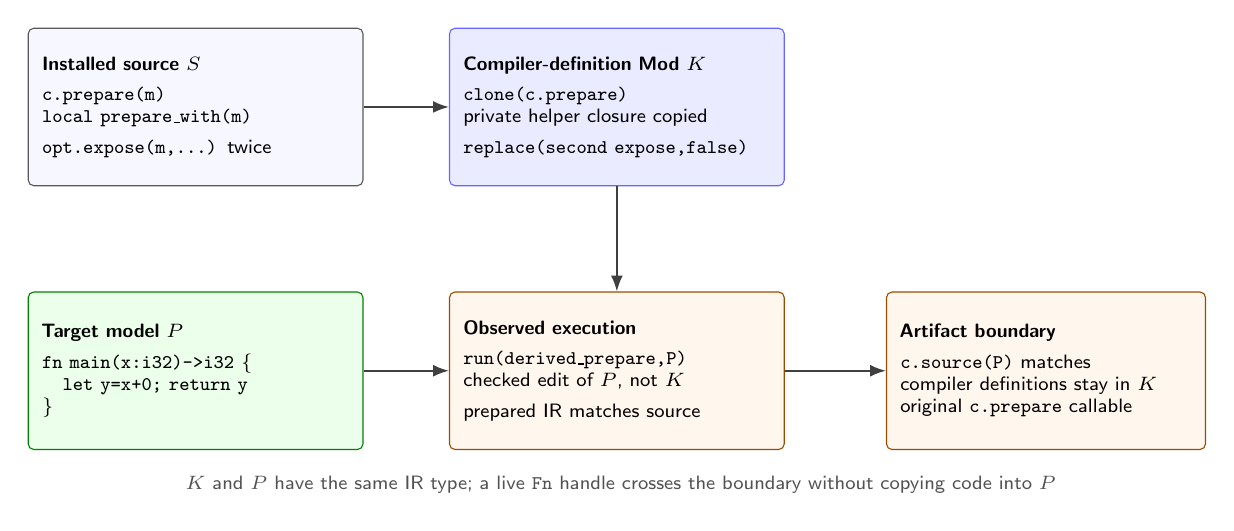
\begin{tikzpicture}[
  body/.style={draw=black!65, rounded corners=2pt, fill=blue!3,
               text width=39mm, minimum height=20mm, align=left,
               inner sep=5pt, font=\sffamily\scriptsize},
  copy/.style={body, fill=blue!8, draw=blue!60},
  subject/.style={body, fill=green!8, draw=green!50!black},
  output/.style={body, fill=orange!7, draw=orange!60!black},
  arrow/.style={-{Latex[length=2mm]}, line width=.65pt, black!75},
  note/.style={font=\sffamily\scriptsize, text=black!68}
]
\node[body] (source) at (0,1.15)
  {\textbf{Installed source $S$}\\[3pt]
   \texttt{c.prepare(m)}\\
   \texttt{local prepare\_with(m)}\\[3pt]
   \texttt{opt.expose(m,...)} twice};
\node[copy] (derived) at (5.35,1.15)
  {\textbf{Compiler-definition Mod $K$}\\[3pt]
   \texttt{clone(c.prepare)}\\
   private helper closure copied\\[3pt]
   \texttt{replace(second expose,false)}};
\draw[arrow] (source) -- (derived);
\node[subject] (model) at (0,-2.2)
  {\textbf{Target model $P$}\\[3pt]
   \texttt{fn main(x:i32)->i32 \{}\\
   \quad\texttt{let y=x+0; return y}\\
   \texttt{\}}};
\node[output] (effect) at (5.35,-2.2)
  {\textbf{Observed execution}\\[3pt]
   \texttt{run(derived\_prepare,P)}\\
   checked edit of $P$, not $K$\\[3pt]
   prepared IR matches source};
\draw[arrow] (derived.south) -- (effect.north);
\draw[arrow] (model) -- (effect);
\node[output, text width=37mm] (artifact) at (10.8,-2.2)
  {\textbf{Artifact boundary}\\[3pt]
   \texttt{c.source(P)} matches\\
   compiler definitions stay in $K$\\
   original \texttt{c.prepare} callable};
\draw[arrow] (effect) -- (artifact);
\node[note] at (5.4,-3.65)
  {$K$ and $P$ have the same IR type; a live \texttt{Fn} handle crosses the boundary without copying code into $P$};
\end{tikzpicture}
\caption{Deriving a real compiler procedure without inserting it into a model.
The source-defined \texttt{c.prepare} wrapper and its private helper closure
are copied to $K$; the second \texttt{opt.expose} call in the copied helper is
replaced with \texttt{false}. On the shown simple typed-model regression, the
edited procedure produces byte-identical prepared IR and C source to the
untouched original. This establishes a valid algorithm-edit path and source
isolation, not general equivalence, faster compilation, or a cross-system
coordination advantage.}
\Description{An installed C preparation function and its private helper are
copied into a separate compiler-definition Mod. A private helper call is
replaced with a constant; a live Fn handle applies the edited procedure to a
separate simple model. Prepared IR and C source match the original on this
regression, while compiler definitions stay outside the model.}
\label{fig:derive}
\end{figure*}

\subsection{Checked choice and transactional change}
Alternative implementations are overloaded functions with structural types.
A selector receives the compatible set and may return at most one member. The
selection mechanism does not prescribe whether the choice is a static rule,
cost model, empirical search, solver, or agent. It does prescribe its authority:
the candidate must be type-compatible, and the resulting program must pass the
same verification and target capability checks.

Mutating module calls execute transactionally. Foreign or stale handles,
non-dominating values, invalid types, and failed verification abort the
invocation and restore the prior program. This property matters for generated
policies and multi-step structural transforms: a failed candidate does not
leave a partially rewritten module for the next candidate or emitter.

\subsection{Artifact closure}
An experiment is complete only when the chosen decisions reach an artifact.
Artifact modules therefore consume the same represented program and derive
external interfaces from exported functions. The C path derives source,
declarations, symbols, buffer shapes, byte counts, and immutable payloads from
one signature model. The application harness consumes the generated descriptor
rather than maintaining a second handwritten ABI. A deterministic virtual
machine provides an independent execution path for semantic and transformation
tests.

Artifact closure exposes rather than hides missing target work. Portable scalar
C is a legal fallback, but its latency reveals absent tiling, packing,
vectorization, library selection, or profitability policy. Those mechanisms can
be added as target modules and evaluated on the same model path.

\section{System realization}
The implementation follows one rule: the host owns validity; modules own
meaning and decisions. Joggle's host is a C++20 library with a textual module
language and embedding API. Its trusted kernel parses and stores
\texttt{Fn/Blk/Op/Val} programs, interns structural types and attributes,
resolves overloads, verifies edits, loads modules, and prints programs
deterministically. It deliberately contains no neural-operator enumeration,
schedule vocabulary, or target lowering table. Adding such a table would turn
the host back into the coordination point that the design is intended to
remove.

\paragraph{One invocation protocol.}
The host resolves every call structurally before execution. Read-only functions
may inspect a frozen revision; mutating functions receive bounded edit
authority. A mutation is staged against that revision, checked for ownership,
liveness, dominance, and type compatibility, and published atomically only
after whole-program verification. Handles carry store identity and generation,
so foreign or stale references fail before an edit is committed. Read-only
functions may use revision-scoped memoization without introducing
process-global analysis state. The protocol is uniform, but the functions are
not: a relation, analysis, selector, transform, and emitter retain different
types and authority.

\paragraph{Modules as linked compiler slices.}
A module packages typed functions, dependencies, visibility, and optionally a
native codec or binding. Installation resolves the dependency closure and all
exported signatures before publishing a new module generation; an upgrade also
checks reverse dependents. Failed validation preserves the installed tree;
commit-phase filesystem errors may require recovery from a retained backup.
Program-edit failure, separately, leaves the prior IR revision intact. This
lifecycle lets a vertical experiment
ship its portable semantics, analyses, policies, and artifact actions together
without granting it unchecked access to the host.

Bundled modules exercise the boundary rather than define privileged cases.
They provide scalar and tensor semantics, ONNX and TFLite bridges, loop and
access analyses, memory planning, C emission, and virtual-machine execution.
Optional codecs decode protobuf and FlatBuffer bytes into source calls; source
names end at the bridge module rather than leaking into tensor or target
modules. Target modules publish capability, preparation, and emission functions
rather than subclasses. The implementation runs under Linux and macOS CI with
address and undefined-behavior sanitizers, while large model artifacts are
checksum-pinned outside the default repository.

\section{Evaluation}
The present evidence establishes prerequisites for malleability rather than the
full revision-cost claim. We separate representational reach, cross-role
extension breadth, generated-code quality, and substrate overhead. Results come
from pinned revisions, models, and inputs with explicit host and thread
contracts and correctness validation. Unsupported, not run, and measured zero
are distinct states; a frontend success is never counted as an executable
artifact. The missing matched evolution study is stated explicitly instead of
being approximated by source size or task completion.

\subsection{RQ1: Does progressive IR survive real models?}
Joggle decodes and infers all fourteen pinned ONNX models and relates thirteen
completely. Table~\ref{tab:models} reports structural frontiers separately from
artifact execution so parsing, inference, or relation is not mislabeled as
deployable support. SSD-MobileNetV1 retains 386 source calls. XCiT-Tiny now
reaches zero source calls, but its C-preparation path expands 3,135 operations
to 18,976 in the first round and does not finish within 227 seconds. The
frontier has therefore moved from frontend semantics to transformation
scalability. Strict generated C passes numerical oracles for ten ONNX models;
the remaining models are not counted as executable support. An official TFLite
MobileNetV2 path independently passes against LiteRT within
$1.1\times10^{-6}$ maximum absolute error.

\begin{table*}[t]
\centering
\caption{Model reach and artifact boundary. ``Unknown'' counts untyped results
after inference; ``calls'' counts source-frontend calls after relation. A check
is a compiled generated-C artifact that passes its numerical oracle; a dash is
not run. XCiT's timeout occurs after complete relation, during C preparation.
Rows are structural and numerical tests, not task-accuracy claims.}
\label{tab:models}
\setlength{\tabcolsep}{6pt}
\begin{tabularx}{\textwidth}{@{}l l r r r r c@{}}
\toprule
Model & Family & Nodes & Tensors & Unknown & Calls & C oracle \\
\midrule
MNIST-8 & classification & 12 & 8 & 0 & 0 & $\checkmark$ \\
MobileNetV2-7 & mobile classification & 155 & 267 & 0 & 0 & $\checkmark$ \\
SqueezeNet1.1-7 & classification & 66 & 53 & 0 & 0 & $\checkmark$ \\
SqueezeNet1.0-13-QDQ & quantized classification & 171 & 229 & 0 & 0 & $\checkmark$ \\
ResNet18-v1-7 & classification & 69 & 102 & 0 & 0 & $\checkmark$ \\
TinyYOLOv2-8 & detection & 33 & 44 & 0 & 0 & $\checkmark$ \\
TinyYOLOv3-11 & detection & 291 & 269 & 0 & 0 & -- \\
UltraFace-RFB-320 & detection & 242 & 244 & 0 & 0 & $\checkmark$ \\
SSD-MobileNetV1-12 & detection & 5,985 & 1,567 & 0 & 386 & -- \\
ShuffleNet-v2-12 & mobile classification & 261 & 282 & 0 & 0 & $\checkmark$ \\
DenseNet-12 & classification & 910 & 848 & 0 & 0 & $\checkmark$ \\
GoogLeNet-12 & classification & 143 & 118 & 0 & 0 & $\checkmark$ \\
EfficientNet-Lite4 INT8 & quantized classification & 97 & 728 & 0 & 0 & -- \\
XCiT-Tiny-12 & vision transformer & 1,310 & 358 & 0 & 0 & prep $>$227 s \\
\bottomrule
\end{tabularx}
\end{table*}

\subsection{RQ2: Can one extension boundary cover distinct compiler roles?}
Table~\ref{tab:extensions} tests role breadth: can the documented extension
path complete four changes that exercise implementation, policy, external
code, and a parameterized numeric format? Joggle completes all four
but through two deliberately distinct paths: the first three are out-of-tree
source modules that require no host change or rebuild, whereas the numeric
format exercises an optional native module and its build target. TVM completes
the first three through
its documented Python/runtime interfaces and preserves an unsupported public
custom-datatype boundary. ONNX-MLIR completes implementation and policy through
an accelerator extension; external-call selection and a second executable
numeric-format target remain unsupported under the frozen contracts. The
controls follow the documented TVM BYOC~\cite{tvmByocDocs} and source-build
~\cite{tvmBuildDocs} interfaces, together with ONNX-MLIR's accelerator
~\cite{onnxmlirAccelDocs} and build~\cite{onnxmlirBuildDocs} interfaces.

The source counts in Table~\ref{tab:extensions} describe the audited surface,
not development effort or usability. The records preserve rebuild scope,
fallback, diagnostic boundary, and final correctness. They do not revise one
vertical concept after the three implementations are frozen, so they establish
role breadth but not lower coordination across revisions. Those dimensions
remain separate rather than being collapsed into an unevidenced ``ease'' score.

\begin{table*}[t]
\centering
\caption{Frozen cross-role extension tasks. P is a complete, oracle-checked
artifact; U is a preserved unsupported boundary; P/U reaches one native target
but not the required second target. Parentheses contain nonblank, noncomment
extension source lines and are descriptive, not an ease metric. S denotes an
out-of-tree source path and N an optional native-module build. Integration is
reported as added build files/registrations; no system changes an existing
framework-core file.}
\label{tab:extensions}
\setlength{\tabcolsep}{7pt}
\begin{tabularx}{\textwidth}{@{}l *{4}{>{\centering\arraybackslash}X} c@{}}
\toprule
System & Implementation & Policy & External kernel & Numeric format & Integration \\
\midrule
Joggle & P/S (20) & P/S (69) & P/S (138) & P/N (284) & 1/0 \\
TVM & P (62) & P (126) & P (355) & U & 0/0 \\
ONNX-MLIR & P (167) & P (201) & U & P/U (516) & 3/1 \\
\bottomrule
\end{tabularx}
\end{table*}

\subsection{RQ3: Can target modules improve complete artifacts?}
The current answer is mixed for transformation reach and negative for
competitive CPU code quality. A general policy rewrites 54 affine-proved
MobileNetV2 bodies through the public module interface. On its preserved
same-runner record, generated-C median latency falls from 139.679 to
102.638\,ms (26.5\%), while the adjacent one-thread ONNX Runtime median is
8.382\,ms. The policy therefore changes a complete, numerically checked
artifact but leaves a 12.24$\times$ gap.

A second complete-artifact probe prevents that result from being read as a
general optimization claim. Greedy loop fusion reduces represented loops from
156 to 110 and C source from 192,209 to 188,244 bytes, yet increases the
MobileNetV2 median from 356.360 to 384.927\,ms on its pinned runner. The
official TFLite path is also numerically correct but records 225.667\,ms for
generated C against 6.424\,ms for one-thread LiteRT. These records use different
shared-runner jobs and are not combined into a cross-row speedup statistic.

The results locate the boundary precisely. Progressive IR and modules can carry
analysis and structural policy into a final artifact; the scalar C target lacks
multi-level tiling, immutable-weight packing, vector and alignment contracts,
library or instruction selection, and a traffic-aware profitability policy.
Malleability makes those mechanisms replaceable. It does not supply them.

\subsection{RQ4: What does the flexibility cost?}
Interpretation and generic structural queries impose visible costs. In a
two-process MobileNetV2 diagnostic, revision-scoped memoization reduces
executed source-function calls from 2,939,981 to 1,272,463 while preserving all
10,008 edits and a byte-identical 28.6-MB result. The corresponding median falls
from 42.099 to 28.341 seconds. A separate indexed-CSE repair reduces one
UltraFace cleanup from 244.26 to 11.28 seconds with the same 597 edits and
byte-identical output. These are unisolated mechanism diagnostics, not
publication-grade throughput measurements.

The remaining boundary is larger than either repair. XCiT preparation grows
from 3,135 to 18,976 operations in its first round and still exceeds 227
seconds. Transaction and stale-handle tests establish atomic failure, but
generative coverage currently reaches parsing and legal IR edit sequences, not
module loading, serialized frontends, or the native ABI. The uniform extension
mechanism is therefore usable on the completed model paths in
Table~\ref{tab:models}, but its large-program scaling and reliability evidence
remain incomplete.

\paragraph{Compiler-definition isolation.}
A mechanism regression exposes a limitation of placing every function in the
model. Copying a compile-time generator into the model to edit it causes C
preparation to encounter compiler-only operations as model work. Holding the
copied \texttt{Fn} in a second \texttt{Mod} of the same IR type lets
\texttt{query} observe its edited output while leaving the model byte-identical.
A copied \texttt{opt.fold\_add\_zero} function then edits the target model
through the direct \texttt{Fn} route; the compiler definition stays unchanged
and the model passes C preparation. Arity, result-type, and read-only failures
retain the prior target revision. This tests execution and artifact isolation;
it does not by itself test an algorithmic change.

A second regression copies the actual \texttt{c.prepare} function with its
transitive private helper closure. The copied \texttt{prepare\_with} body is
edited so its second \texttt{opt.expose} call returns \texttt{false}. The code
module verifies, and the original function remains callable. The pilot extends
that check to complete ONNX and TFLite MobileNetV2 semantic programs and prior
canonical UltraFace and SqueezeNet programs. For each, the original and derived
procedures produce byte-identical prepared IR and generated C source; both
outputs verify. The MobileNet programs move through 7,593 and 9,866 structural
revisions, respectively. A phase trace confirms that the first
\texttt{opt.expose} performs edits, whereas the second performs no structural
edit on any of these four inputs. The TFLite type-inference stage still changes
the model revision between the calls. The copied compiler definition contains
20 functions and 1,115 operations. Thus the experiment establishes isolated
execution of an edited compiler procedure on real models, but the particular
edit removes work that was already inactive in the observed inputs. It does
not establish a generally legal rewrite or a speedup; the unisolated macOS
times are diagnostic only. A matched mechanism control remains necessary.

\section{Related work}
\subsection{Extensible compiler construction}
Compiler extensibility is an old goal, but prior systems choose different units
of change. JastAdd and Polyglot modularize language extensions and analyses
~\cite{ekman2007jastadd,nystrom2003polyglot}. Spoofax is the closest lifecycle
precedent: one textual language project composes syntax modules and reuses a
semantic description across analysis, transformation, code generation, and
editor services~\cite{kats2010spoofax}. Cross-role packaging is therefore not
new by itself. Nanopass makes the compiler a sequence of small languages, Magik
loads application semantics over compiler IR, and LMS composes staged DSLs
through horizontal extensions and vertical transformations
~\cite{sarkar2005nanopass,engler1997magik,rompf2016lms}.

Joggle moves the language-workbench idea to a different mutable object and
failure boundary. Its modules execute typed analyses and transactional edits
over a live compiler program, participate in target selection, construct native
artifacts, and are checked with reverse dependents before an upgrade is
published. The claim is not the existence of modules or reusable semantic
definitions; it is their coupling to progressive function exposure, checked
module replacement, and verified program-edit transactions.

Recent work gives module semantics directly to IR. \cite{klopp2024datalogmodules}
provides statically typed, separately compiled modules, explicit required and
provided relations, partial linking, and bundles. This is the nearest formal
module comparison. Its modules organize Datalog relations and are linked before
ordinary compiler passes; Joggle modules additionally execute typed analyses
and transactional edits over live IR and construct external artifacts. The
resolver and upgrade semantics are therefore part of compilation, not
incidental package tooling.

\cite{fehr2023xdsl} takes a complementary sidekick approach: it recreates
MLIR-compatible SSA infrastructure in Python and exchanges textual IR and
declarative definitions with the production ecosystem. MLIR itself supports
runtime-defined dialects, IRDL vocabulary, external interface models, and
partial conversion
~\cite{mlirDynamicDialectDocs,mlirIrdlDocs,mlirInterfacesDocs,mlirConversionDocs}. Its Transform
dialect exposes precise, composable compiler transformations, preconditions,
postconditions, and search integration as transform IR without requiring a
custom pass for each policy~\cite{lucke2025transform,mlirTransformDocs}. These are close
comparisons for research accessibility and controllable compilation. Joggle
uses ordinary \texttt{Fn} bodies for model meaning and compiler procedures.
An inactive compiler definition can be copied, edited, and invoked over a
separate model value. The question is whether this reduces the integration
cost of useful derived procedures across compiler roles while retaining
Transform's explicit checks. The current regression establishes execution,
not that comparative consequence.

AnyDSL uses online partial evaluation and higher-order functions known to the
compiler to specialize generic algorithms for CPUs and GPUs
~\cite{leissa2018anydsl}. Weval derives compiled execution from an existing
interpreter function under explicit specialization promises
~\cite{fallin2025weval}. Exo 2 permits users to build new scheduling operations
from trusted primitives~\cite{ikarashi2024exo2}. These works already make
optimization procedures programmable or derivable. Joggle's claim must
therefore be tested across analysis, policy, representation, and artifact
behavior rather than inferred from \texttt{clone} or \texttt{invoke} alone.

TVM's runtime and \texttt{PackedFunc} API is the strongest counterexample
to a uniform-call claim~\cite{tvmRuntimeDocs}: TVM deliberately uses the same
type-erased callable for compiler passes,
frontend callbacks, compiled functions, device modules, and RPC. Joggle chooses
a different contract. Calls are structurally typed before execution, module
source may define both portable semantics and compiler actions, mutations are
transactional, and package upgrade checks bindings in reverse dependents.
Consequently, one function syntax is not evidence by itself; the claimed
difference lies in structural checking, atomic mutation, and dependency-safe
replacement.

\subsection{Multi-level composition and deployment}
Specialized IR boundaries solve real optimization problems. TVM's
\texttt{IRModule} already composes high-level Relax functions, low-level
\texttt{PrimFunc}s, and external calls; shared types and cross-level passes make
this substantially more than a fixed lowering pipeline
~\cite{lai2025relax,tvmArchitectureDocs}. MLIR's generic
\texttt{Operation}, \texttt{Region}, \texttt{Block}, and \texttt{Value}
storage already permit heterogeneous
dialects in one program; local coexistence and a common edit model are not
Joggle inventions~\cite{mlirLangRefDocs,mlirConversionDocs}. Its Transform
dialect represents fine-grained control as transform IR over the payload
~\cite{lattner2021mlir,lucke2025transform,mlirTransformDocs}. ONNX-MLIR uses MLIR for
ONNX-to-native compilation~\cite{jin2020onnxmlir}; IREE connects such pipelines
to a low-overhead AOT runtime~\cite{ireeDocs}. Joggle does not argue that these
abstraction boundaries should collapse, nor that its scheduler is richer.

The narrower distinction is the proposed \emph{unit of independently governed
change}. An MLIR project can combine IRDL definitions, external interfaces,
conversion patterns, transform operations, passes, and runtime code; TVM can
compose Relax, TensorIR, and runtime modules. Joggle makes one installed typed
source module the dependency unit spanning portable semantics, inspection,
selection, guarded IR mutation, and artifact actions, while a consumer requests
local exposure only when its accepted capability requires it. A procedure may
be derived in a separate \texttt{Mod} value and applied through a live
function handle. This does not prove fewer contracts or lower engineering
cost. A matched revision path or procedure-derivation study with comparable
coordination and execution cost in MLIR or Relax would falsify Joggle's
central advantage.

\subsection{Controllable tensor and kernel construction}
Lift, RISE, and Elevate make transformation strategy explicit in functional
languages~\cite{steuwer2017lift,steuwer2022rise}. Halide and Tiramisu separate
algorithms from schedules~\cite{ragankelley2013halide,baghdadi2019tiramisu}.
TensorIR, Hidet, and TileLang expose different combinations of blocks, tiles,
threads, data movement, and mapping
~\cite{feng2023tensorir,ding2023hidet,wang2025tilelang}. Exo goes further by
externalizing target instructions, specialized memories, configuration state,
and trusted schedule rewrites into user code~\cite{ikarashi2022exo}. Sparse and
heterogeneous systems similarly make format, data movement, or custom-type
choices explicit~\cite{daghero2025sparse}.

These systems provide richer scheduling and kernel construction than Joggle.
Joggle addresses the orthogonal lifecycle around a kernel: model recognition,
portable fallback, policy substitution, validation, and artifact closure remain
connected while an implementation changes. This does not waive matched
kernel-quality comparison; it identifies where their scheduling or search
mechanisms can enter the Joggle path.

\subsection{Automatic optimization and backend construction}
Ansor searches tensor programs; Roller constrains shapes to hardware-friendly
tiles; Welder jointly schedules operators through a tile graph; Ladder couples
custom datatypes with storage, access, conversion, and scheduling
~\cite{zheng2020ansor,zhu2022roller,shi2023welder,wang2024ladder}. TASO, Tensat,
Glenside, Mirage, and Axon enlarge the transformation space through generated
substitutions, equality saturation, access-pattern rewriting, or multi-level
superoptimization
~\cite{jia2019taso,yang2021tensat,smith2021glenside,wu2024mirage,kothari2026axon}.
ACT generates instruction selection and scratchpad allocation from tensor-ISA
semantics, while ATLAAS lifts RTL behavior toward those specifications
~\cite{jain2026act,gao2026atlaas}.

Joggle contributes none of these search or synthesis algorithms. It supplies a
checked control plane through which a handwritten rule, bounded search,
synthesizer, or generated policy can propose alternatives without changing the
surrounding execution and artifact path. Selector substitution isolates this
composition claim from optimizer quality.

\subsection{Hardware--representation co-design and edge inference}
DORY, MCUNet, Ladder, and recent sparse-MCU systems show that datatype,
encoding, memory organization, kernels, compiler integration, and model choice
can be one systems result
~\cite{burrello2021dory,lin2020mcunet,wang2024ladder,daghero2025sparse}.
TensorFlow Lite Micro, ncnn, and IREE establish stronger baselines for runtime
breadth, tuned kernels, memory planning, and deployable artifacts
~\cite{david2021tflm,ncnnProject,ireeDocs}. FlashInfer shows the same vertical
pressure in modern attention: cache representation, kernel templates, JIT
specialization, and runtime scheduling interact~\cite{ye2025flashinfer}.

Joggle uses edge inference as a demanding evaluation domain, not as a claim of
edge-only applicability. Mechanism generality is evaluated by whether portable
and specialized policies share the same extension path; implementation maturity
is separately evaluated by model coverage, correctness, latency, memory,
compile time, and artifact size.

\subsection{Generated policies and compiler reliability}
LLM-aided optimizers generate mappings or kernels but depend on compilers,
profilers, and correctness oracles to admit results
~\cite{hong2025autocomp,mai2026argus}. NNSmith, HirGen, compiler bug studies,
and metamorphic testing show that broad operator support and complex
transformation stacks create a large semantic failure surface
~\cite{liu2023nnsmith,ma2023hirgen,zheng2021compilerbugs,xiao2022metamorphic}.
Joggle's transactional edits and explicit frontiers are relevant only if they
reject invalid proposals early, preserve working paths, and produce
reproducible diagnostics; these properties are measured rather than inferred
from API design.

\section{Discussion and limitations}
Progressive IR is not a universal replacement for multi-level IR. A
specialized representation is preferable when its invariants enable analyses
or transformations that cannot be expressed economically over Joggle's public
structure. Dynamic shapes, stateful model execution, device concurrency, and
distributed placement are not yet mature. The current C target is transparent
but lacks the tuned kernels and vector machinery of production systems.

Joggle instead targets the phase in which a model or hardware mechanism is
still changing. Its success criterion is that researchers can package general
compiler logic and specialized machine decisions together, revise them without
central cases, and measure the resulting artifact. Broader deployment support
and competitive performance remain empirical obligations, not consequences of
the architecture.

Procedure derivation has its own cost boundary. Keeping snapshots of edited
compiler bodies by source revision fixes stale execution, but repeated
procedure revisions may increase interpretation-cache memory. Typed
verification checks structural integrity; preservation of an analysis result
or transformation effect requires an algorithm-specific argument or oracle.
Native procedures remain opaque to function-body edits. These boundaries
belong in a comparison with MLIR Transform, staging, or a compiled compiler
implementation.

\section{Conclusion}
Joggle uses a progressive function representation for both model computation
and source-defined compiler procedures. Typed modules keep analyses, choices,
structural edits, and generation inspectable, while separate values of the
same \texttt{Mod} type let a derived procedure act on a model without becoming
part of its artifact. Current complete-model evidence establishes semantic
and artifact reach but also a large gap to production runtimes. A matched
revision or useful procedure-derivation comparison remains the decisive test
of the claimed compilation benefit.

\bibliographystyle{ACM-Reference-Format}
\balance
\bibliography{../references}
\end{document}
